% !TEX root = ../main.tex
\subsubsection{Central Detector}
\label{sssec::central_detector}
    In the CLAS12 Central Detector (CD), particles scattered from the target within the polar angle range of $35\degree$ to $125\degree$ are detected.
    The CD consists of various detectors that provide particle identification and tracking capabilities.
    Charged particles are detected in the Central Vertex Tracker (CVT) and the Central Time-of-Flight (CTOF) detector.
    Neutron detection is provided by the Central Neutron Detector (CND), which is located radially outside of the CVT and the CTOF.
    All detectors have full coverage in the azimuthal angle.

    % !TEX root = ../main.tex
\paragraph{Central Vertex Tracker (CVT)}
    The CVT system is an integral part of the CD.
    It is primarily used for measuring the momentum and determining the vertex position of charged particles scattered from the target.

    The CVT system is located inside the solenoid magnet, as depicted in Figure \ref{fig::11.221::cvt}.
    It consists of two distinct detectors: the SVT and the Barrel Micromegas Tracker (BMT).

    The SVT system is composed of three regions, each equipped with double-sided modules of silicon sensors.
    The regions have different numbers of modules: 10, 14, and 18, respectively.
    These silicon sensors are instrumented with a digital Application-Specific Integrated Circuit (ASIC) readout.
    The readout pitch, which refers to the distance between adjacent readout channels, is approximately 156 micrometers.
    The SVT system comprises 21,504 channels \cite{antonioli2020}.

    \begin{wrapfigure}{r}{0.50\textwidth}
        \frame{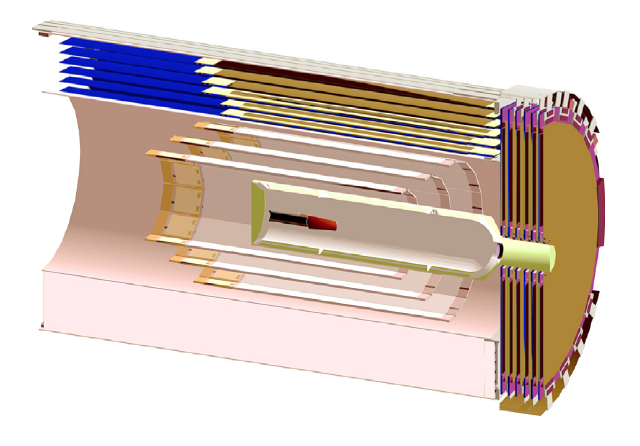
\includegraphics[width=\linewidth]{221cvt.png}}
        \caption[Central Vertex Tracker (CVT)]
        {Render of the Central Vertex Tracker (CVT).
        From the inside, the figure shows the target cell and vacuum chamber, the three double layers of the SVT, followed by the six layers of the BMT.
        The beam enters from the left.
        The six Forward Micromegas Tracker (FMT) layers are shown at the downstream end at the right.}
        \floatfoot{Source: \href{https://jlab.org/physics/hall-b/clas12}{CLAS12 wiki}.}
        \label{fig::11.221::cvt}
    \end{wrapfigure}

    The BMT is composed of three layers of strips aligned along the beamline and three layers of circular readout strips around the beamline, totalling 15,000 readout elements.
    It significantly enhances momentum resolution and tracking efficiency.
    Each layer is divided azimuthally into three segments, providing $120\degree$ azimuthal coverage for each segment.
    The system is designed to operate at the full luminosity of $10^{35} \text{cm}^{-2}\text{s}^{-1}$ \cite{acker2020mvt}.

    % !TEX root = ../main.tex
\paragraph{Central Time-of-Flight}
    The CTOF system is utilised for the purpose of charged particle identification by measuring their time-of-flight (TOF) in the momentum range of approximately $0.3$ to $1.25 ~\text{GeV}$.
    It consists of 48 plastic scintillators with double-sided photomultiplier tube (PMT) readout.
    The PMTs are connected to the scintillators via 1.0-meter-long upstream and 1.6-meter-long downstream focusing light guides.
    These counters are arranged in a hermetic barrel configuration surrounding the target and the CVT, and they are aligned with the beam axis inside the 5 T solenoid magnet.

    To ensure accurate measurements, the PMTs are positioned within a region of 0.1 T fringe field of the solenoid magnet and are enclosed within a triple-layer dynamic magnetic shield.
    This shield minimises the internal magnetic field near the PMT photocathode, achieving a field strength of less than 0.2 G.
    The CTOF system is designed to provide a time resolution of 80 ps, enabling precise charged particle identification in the CLAS12 CD \cite{carman2020ctof}.

    For a visual representation of the CTOF system, you can refer to figure \ref{fig::ctof}.

    % !TEX root = ../main.tex
\paragraph{Central Neutron Detector (CND)}
    The Central Neutron Detector (CND) is a component of the CLAS12 Central Detector (CD) positioned radially outward of the CTOF system.
    Its primary function is to detect neutrons in the momentum range of $0.2$ to $1.0 \text{GeV}$ by measuring their TOF from the target and the energy deposition in scintillator layers.

    The CND is composed of three layers of scintillator paddles, with each layer containing 48 paddles.
    The paddles are coupled in pairs at the downstream end using semi-circular light guides.
    The signal generated in the scintillator paddles is read out at the upstream end by PMTs that are positioned outside the high magnetic field region of the solenoid magnet.

    To transmit the scintillation light, the scintillators are connected to 1-meter-long bent light guides, which ensure efficient light propagation to the PMTs for signal detection and readout.

    The combination of TOF measurements and energy deposition in the scintillator layers enables the CND to identify and detect neutrons within the specified momentum range in the CLAS12 CD \cite{chatagnon2020}.

    % !TEX root = ../main.tex
\paragraph{Back Angle Neutron Detector (BAND)}
\label{par::band}
    \begin{wrapfigure}{r}{0.49\textwidth}
        \centering\frame{
        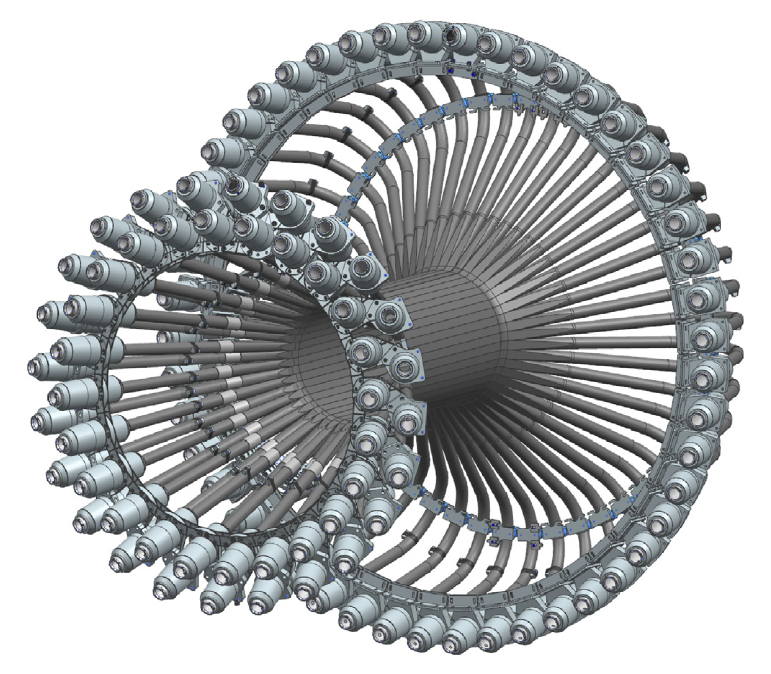
\includegraphics[width=\linewidth]{222ctof.png}}
        \caption[Central Time-of-Flight]{Render of the Central Time-of-Flight.
        The render shows CTOF's 48 scintillator bars outfitted with light guides, PMTs, and magnetic shields at both ends of each counter.
        Source: \hyperlink{https://www.jlab.org/physics/hall-b/clas12}{CLAS12 wiki}.}
        \label{fig::ctof}
    \end{wrapfigure}

    The CLAS12 spectrometer includes the BAND as a dedicated detector for neutron detection at backward angles.
    Positioned 3 metres upstream of the target, the BAND is designed to detect backward-scattered neutrons with momenta ranging from 0.25 to 0.7 GeV.

    The BAND detector consists of 18 horizontal rows and five layers of scintillator bars.
    Each scintillator bar is equipped with PMT readout on both ends to measure the TOF of neutrons originating from the target.
    Additionally, there is an extra 1 cm scintillation layer specifically designed to veto charged particles, ensuring that only neutrons are detected.

    Covering a polar angle range from $155\degree$ to $175\degree$, the BAND detector achieves a design neutron detection efficiency of $35\%$.
    It also provides a momentum resolution of approximately $1.5\%$, allowing for precise measurements of the momentum of the detected neutrons \cite{segarra2020}.

    By utilising the BAND detector, the CLAS12 spectrometer is capable of detecting and characterising backward-scattered neutrons, providing valuable information for various physics studies and experiments conducted at CLAS12.

